\documentclass[10pt]{beamer}
%\usepackage[french]{babel}

\usetheme{metropolis}
\usepackage{appendixnumberbeamer}

\usepackage{booktabs}
\usepackage[scale=2]{ccicons}


\usepackage{natbib}

\usepackage{pgfplots}
\usepgfplotslibrary{dateplot}

\usepackage{rotating}


\usepackage{xcolor} 

%\usepackage{subcaption}

%\usepackage{floatrow}

\usepackage{dsfont}
\usepackage{bm}

%\usepackage[font=small,skip=0pt]{caption}

\usepackage{xspace}
\newcommand{\themename}{\textbf{\textsc{metropolis}}\xspace}

\usepackage{amsmath}
\usepackage{amssymb}
\usepackage{centernot}

\usepackage{multicol}

\usepackage{fancyvrb} 
\DefineVerbatimEnvironment{rcode}{Verbatim}{fontsize=\scriptsize,formatcom={\color{brown}}} % avec fancyvrb
\DefineVerbatimEnvironment{rcoderouge}{Verbatim}{fontsize=\scriptsize,formatcom={\color{red}}} % avec fancyvrb


\usepackage{tikz}
\usetikzlibrary{calc}

\newcommand{\tikzmark}[1]{\tikz[overlay,remember picture] \node (#1) {};}
\newcommand{\DrawLine}[3][]{%
    \begin{tikzpicture}[overlay,remember picture]
        \draw [#1] ($(#2)+(0,0.6ex)$) -- ($(#3)+(0,0.6ex)$);
    \end{tikzpicture}%
}% cross out row in a table

\DeclareMathOperator{\sinc}{\mathrm{sinc}}

\DeclareMathOperator*{\argmin}{arg\,min}
\DeclareMathOperator*{\argmax}{arg\,max}

\newcommand\independent{\protect\mathpalette{\protect\independenT}{\perp}} % define independent symbol
\def\independenT#1#2{\mathrel{\rlap{$#1#2$}\mkern2mu{#1#2}}}


\newcommand*{\QEDA}{\hfill\ensuremath{\blacksquare}}%
\newcommand*{\QEDB}{\hfill\ensuremath{\square}}%

\usepackage{xcolor}
\definecolor{definitionBlue}{HTML}{447EB4}



\newcommand{\blue}[1]{\textcolor{blue}{#1}}
\newcommand{\Norm}[1]{\left\lVert#1\right\rVert}
\newcommand{\rank}[1]{\operatorname{rank}\p{#1}}
\newcommand{\p}[1]{\left(#1\right)}
\newcommand{\pink}[1]{\textcolor{pink}{#1}}
\newcommand{\red}[1]{\textcolor{red}{#1}}
\newcommand{\simiid}{\,{\buildrel \text{iid} \over \sim\,}}
\newcommand{\nn}{\mathcal{N}}
\newcommand{\prob}[1]{\mathbb{P}\left(#1\right)}
\def\by{y}
\def\bx{x}
\def\bz{z}
\def\bbeta{\beta}
\def\like{{\cal L}}
\def\llike{{\cal LL}}
\newcommand{\dens}{\texttt{p}}
\def\iid{\mathop{\sim}_{\rm i.i.d.}}
\def\ximis{\bx_{i,{\rm mis}}}
\def\xiobs{\bx_{i,{\rm obs}}}
\def\xmis{\bx_{{\rm mis}}}
\def\xobs{\bx_{{\rm obs}}}
\def\xa{\bx^{(\rm mis)}}
\def\xb{\bx^{({\rm obs})}}
\def\thml{\hat{\theta}_{\rm ML}}




% Note, that you have to have Mozilla's \emph{Fira Sans} font and XeTeX installed to enjoy this wonderful typography.

\title{\large Data Challenge pour les SHS}
\subtitle{\small Analyse de données et introduction aux méthodes d'apprentissage automatique}

%\author{Julie Josse}
%\institute{EHESS; \'Ecole Polytechnique; Stanford Business School; Traumabase$^{\tiny{\textregistered}}$ \,Group}

\date{Lundi 18 Janvier 2021}

% \titlegraphic{\hfill\includegraphics[height=1.5cm]{logo.pdf}}

\begin{document}
%\nocite{*}

%\maketitle

%\begin{frame}{Outline}
  \setbeamertemplate{section in toc}[sections numbered]
%  \tableofcontents[hideallsubsections]
%\end{frame}

\frame{\titlepage
}
% Avec cette commande au d�but du document,
% le plan sera rappel� � chaque changement de section

%\frame{\frametitle{Research activities}
%
%
%\vfill
%\begin{itemize}
%\item Dimensionality reduction methods to visualize complex data 
%(PCA based): multi-sources, textual, arrays, questionnaire
%\item Low rank estimation, selection of regularization parameters
%\item Missing values - matrix completion
%\item Causal inference
%\vfill
%\vfill
%\item Fields of application: bio-sciences (agronomy, sensory analysis), health data (hospital data)
%\vfill
%\vfill
%\item R community: book R for Stat, R foundation, taskforce,  packages:
%\vfill
%\small{
%\href{http://factominer.free.fr/}{\blue{FactoMineR}}
%\small{explore continuous, categorical, multiple contingency tables (correspondence analysis), combine clustering and PC, .. }\\ \normalsize 
%\href{http://juliejosse.com/wp-content/uploads/2015/11/jss1451.pdf}{\blue{MissMDA}} 
%\small{for single and multiple imputation, PCA with missing} \normalsize\\
%\href{https://github.com/julierennes/denoiseR} {\blue{denoiseR}} \small{to denoise data with low-rank estimation} \\ \normalsize 
%\href{https://github.com/R-miss-tastic} {\blue{R-miss-tastic}} 
%\small{missing values plateform} \normalsize\\
%
%
%\normalsize
%
%
%}\normalsize
%\end{itemize}
%}

%\begin{frame}
%\frametitle{Overview} % Table of contents slide, comment this block out to remove it
%\tableofcontents % Throughout your presentation, if you choose to use \section{} and \subsection{} commands, these will automatically be printed on this slide as an overview of your presentation
%\end{frame}



%\frame{\frametitle{Collaborators}
%\vfill
%\textbf{Jean-Pierre Nadal (ENS-EHESS), Stefan Wager (Stanford)}, Wei Jiang (X), Nicolas Prost (X) \\
%Traumabase (APHP): Tobias Gauss, Sophie Hamada, Jean-Denis Moyer    \\
%Capgemini
%\vfill
%
%
%\begin{center}
%\includegraphics[width=0.14\textwidth]{pic/josse.jpg} ~
%\includegraphics[width=0.14\textwidth]{pic/nadal.jpg} ~
%\includegraphics[width=0.14\textwidth]{pic/wager.jpg} ~
%\includegraphics[width=0.14\textwidth]{pic/jiang.jpg}  ~
%\includegraphics[width=0.14\textwidth]{pic/gauss.jpg} ~
%\includegraphics[width=0.14\textwidth]{pic/hamada.jpg} 
%\end{center}
%\vfill
%\begin{center}
%\includegraphics[width=0.13\textwidth]{pic/polytechnique.png} \hspace{1cm}
%\includegraphics[width=0.17\textwidth]{pic/ehess.png}  \hspace{1cm}
%\includegraphics[width=0.3\textwidth]{pic/aphp.jpg} 
%\end{center}
%\vfill
%
%}







%%%%%%%%%%%%%%%%%%%%%%%%%%%%
\frame
%%%%%%%%%%%%%%%%%%%%%%%%%%%%
{ \frametitle{Data Challenge pour les SHS}
\vfill
\vspace{0.1cm }
\textbf{Objectifs du cours}: Se doter d'outils statistiques et de visualisation pour analyser un jeu de données. Aborder les méthodes modernes d'apprentissage automatique par l'application, et en percevoir les forces et les limites.\\
\vspace{0.1cm }
\pause
\textbf{Programme}
\begin{enumerate}
\item Cours 1: Visualisation de données et statistiques descriptives (\texttt{R})
\item Cours 2 \& 3: Réduction de dimension, ACP, et clustering (\texttt{R})
\item Cours 4: Régression (\texttt{R})
\item Cours 5 \& 6: Modèles prédictifs (\texttt{Python} et \texttt{scikit-learn})
\item Cours 7: Modèles prédictifs avancés dont analyse de texte et introduction au \textit{deep learning} (\texttt{Python})
\item Et des séances dédiées au projet intercallées entre les cours
\end{enumerate}

\vfill
}


%%%%%%%%%%%%%%%%%%%%%%%%%%%%
\frame
%%%%%%%%%%%%%%%%%%%%%%%%%%%%
{ \frametitle{Langages utilisés}

\textbf{Nous utiliserons \texttt{R} et \texttt{Python} pendant ce cours}

\vspace{0.2cm}

    \begin{columns}[T] % align columns
    \begin{column}{.48\textwidth}
    \color{cyan}\rule{\linewidth}{2pt}
    
    \texttt{R}
    \vspace{0.5cm}
    \begin{itemize}
        \item Environnement: RStudio
        \vspace{0.2cm}
        \item Outils utilisés:
        \begin{itemize}
            \item Visualisation (\texttt{ggplot2})
            \item Régression (\texttt{glm})
            \item Analyse en composantes principales (\texttt{FactoMineR})
        \end{itemize}
      \end{itemize}
      \vspace{0.5cm}
       Cours 1, 2, 3, et 4
    \end{column}%
    \hfill%
    \begin{column}{.48\textwidth}
    \color{orange}\rule{\linewidth}{2pt}
    
    \texttt{Python}
    \vspace{0.5cm}
    \begin{itemize}
        \item Environnement: Jupyter
        \vspace{0.2cm}
        
        \item Outils utilisés:
        \begin{itemize}
            \item \textit{Machine learning} avec \texttt{scikit-learn})
            \item Analyse de texte avec \texttt{FastText}
        \end{itemize}
    \end{itemize}
    \vspace{0.5cm}
    Cours 5, 6 et 7
    \end{column}%
    \end{columns}

}

%%%%%%%%%%%%%%%%%%%%%%%%%%%%
\frame
%%%%%%%%%%%%%%%%%%%%%%%%%%%%
{ \frametitle{Organisation et intervenants}
\textbf{Intervenants}\\


Les cours seront assurés alternativement par Bénédicte Colnet, Julie Josse, Gaël Varoquaux et les TDs par Bénédicte (doctorante à Inria).

\vspace{0.5cm}
\begin{columns}
\begin{column}{.45\linewidth}\centering
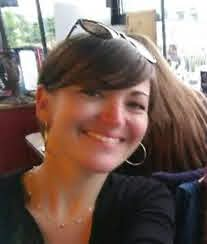
\includegraphics[width=2.3cm]{juliejosse}\par 
Julie Josse \\ Advanced Researcher (Inria)
\end{column}
\begin{column}{.45\linewidth}\centering
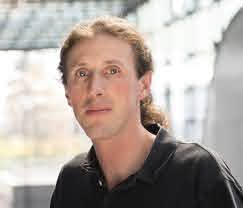
\includegraphics[width=3cm]{gaelvaroquaux}\par 
Gaël Varoquaux\\ Research director (Inria)
\end{column}

\end{columns}


\textbf{Comité de pilotage}\\
Julie Josse (Ecole Polytechnique, Inria), Jean-Pierre Nadal (CAMS, CNRS \& EHESS), Gaël Varoquaux (Inria), et Annick Vignes (CAMS,  Irstea)
}

%%%%%%%%%%%%%%%%%%%%%%%%%%%%
\frame
%%%%%%%%%%%%%%%%%%%%%%%%%%%%
{ \frametitle{Évaluation par projet}

\textbf{Objectifs}\\
Appliquer les méthodes vues en cours, et commencer par des étapes d’exploration, visualisation des données, puis des modélisations en utilisant les méthodes/algorithmes nécessaires pour répondre à la question (en insistant sur les compromis pouvoir prédictif/interprétabilité, la nécessité de toujours se comparer à des méthodes simples, etc). 

\textbf{Sujet}\\
Proposition des différents sujets dans 3 semaines. 

\begin{quote}
N.B.: Vous pouvez éventuellement proposer un sujet (en lien avec vos intérêts, ou un autre projet de recherche, ou encore suite à une lecture)! Il vous faudra cependant déjà des données. Dans ce cas contactez nous avec votre proposition.
\end{quote}


\textbf{Rendu}\\
Présentation orale (10min) et rapport sur les résultats (10 pages)

}


%%%%%%%%%%%%%%%%%%%%%%%%%%%%
\frame
%%%%%%%%%%%%%%%%%%%%%%%%%%%%
{ \frametitle{Informations pratiques}

\begin{itemize}

\item Language: Français pendant le cours, mais les slides et notebooks seront en anglais.
\item Horaires: Lundi 10h-12h, 18 janvier (B. Colnet), 25 janvier (J. Josse), 1 Février (B. Colnet), 8 Février (B. Colnet),  15 Février (G. Varoquaux), 22 Février (G. Varoquaux), [Pas de cours le 1er Mars], 8 Mars (G. Varoquaux), 15 Mars, 22 Mars, 29 Mars (un cours d'économétrie avec Annick Vignes est prévu)
\item Contact: benedicte.colnet@inria.fr \\ Ne pas hésiter pour toute question. Nous pourrons aussi mettre en place un slack ou bien une permanence selon les besoins. 
\vfill

\item L'évaluation se fait 100\% sur le projet. 

\item Prérequis: Il est fortement conseillé d'effectuer en amont l'installation et la prise en main des outils \texttt{R} et \texttt{Python} que nous allons utiliser pour les étudiants n'ayant jamais utilisé ces outils. \\

\end{itemize}
}

\end{document}

